\documentclass[border=15pt, multi, tikz]{standalone}

\usepackage{tikz}
\usetikzlibrary{quotes,arrows.meta}
\usetikzlibrary{positioning}
\def\edgecolor{rgb:blue,4;red,1;green,4;black,3}
\newcommand{\midarrow}{\tikz \draw[-Stealth,line width =0.8mm,draw=\edgecolor] (-0.3,0) -- ++(0.3,0);}
\usepackage{Box}
\usepackage{RightBandedBox}

\def\ConvColor{rgb:blue,5;green,2.5;white,5}
\def\ConvReluColor{rgb:blue,5;green,5;white,5}
\def\PoolColor{rgb:red,1;black,0.3}
\def\DcnvColor{rgb:blue,5;green,2.5;white,5}
\def\UnpoolColor{rgb:yellow,5;red,2.5;white,5}
\def\SoftmaxColor{rgb:magenta,5;black,7}

\usetikzlibrary{3d} %for including external image 

\begin{document}

\begin{tikzpicture}
\tikzstyle{connection}=[ultra thick,every node/.style={sloped,allow upside down},draw=\edgecolor,opacity=0.7]
%%%%%%%%%%%%%%%%%%%%%%%%%%%%%%%%%%%%%%%%%%%%%%%%%%%%%%%%%%%%%%%%%%%%%%%%%%%%%%%%%%%%%%%%
%% Draw Layer Blocks
%%%%%%%%%%%%%%%%%%%%%%%%%%%%%%%%%%%%%%%%%%%%%%%%%%%%%%%%%%%%%%%%%%%%%%%%%%%%%%%%%%%%%%%%
%%%%%%%%%%   
\node[canvas is zy plane at x=0] (alan) at (0,0,0) {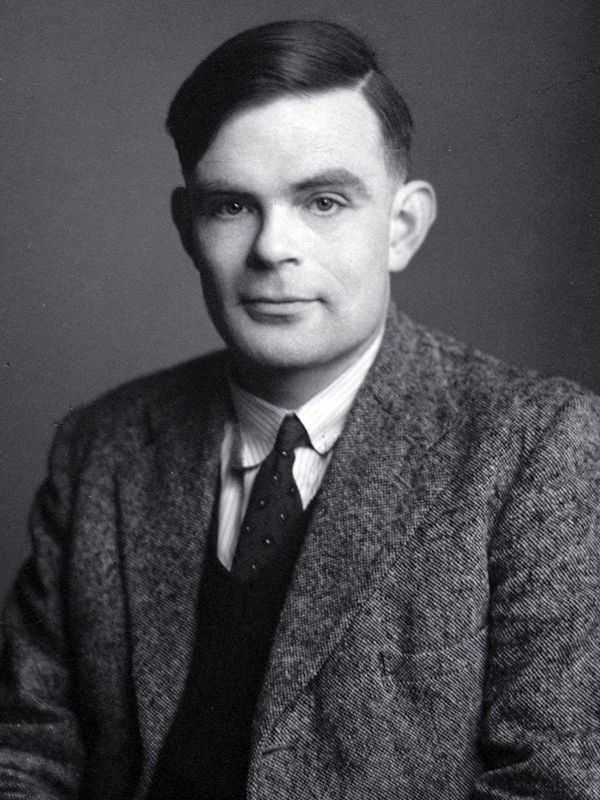
\includegraphics[width=9cm,height=9cm]{img/alan-turing.jpg}};


% CONVOLUTION
\pic[shift={(4,0,0)}] at (alan) {RightBandedBox={name=c1,caption=CONVOLUTION,
        fill=\ConvColor,bandfill=\ConvReluColor,
        height=40,width={2,2,2,2,2},depth=40}};
% POOLING
\pic[shift={(3,0,0)}] at (c1-east) {RightBandedBox={name=p1,caption=POOLING,
        fill=\PoolColor, height=20,width={2,2,2,2,2},depth=20}};

% CONVOLUTION
\pic[shift={(3,0,0)}] at (p1-east) {RightBandedBox={name=c2,caption=CONVOLUTION,
        fill=\ConvColor,bandfill=\ConvReluColor,
        height=20,width={2,2,2,2,2},depth=20}};
% POOLING
\pic[shift={(3,0,0)}] at (c2-east) {RightBandedBox={name=p2,caption=POOLING,
        fill=\PoolColor, height=10,width={2,2,2,2,2},depth=10}};

% CONVOLUTION
\pic[shift={(3,0,0)}] at (p2-east) {RightBandedBox={name=c3,caption=CONVOLUTION,
        fill=\ConvColor,bandfill=\ConvReluColor,
        height=10,width={2,2,2,2,2},depth=10}};

% unPOOLING
\pic[shift={(3,0,0)}] at (c3-east) {RightBandedBox={name=up1,caption=UPSAMPLING,
        fill=\UnpoolColor, height=20,width={2,2,2,2,2},depth=20}};

% CONVOLUTION
\pic[shift={(3,0,0)}] at (up1-east) {RightBandedBox={name=c4,caption=CONVOLUTION,
        fill=\ConvColor,bandfill=\ConvReluColor,
        height=20,width={2,2,2,2,2},depth=20}};
        
% unPOOLING
\pic[shift={(3,0,0)}] at (c4-east) {RightBandedBox={name=up2,caption=UPSAMPLING,
        fill=\UnpoolColor, height=40,width={2,2,2,2,2},depth=40}};

% CONVOLUTION
\pic[shift={(3,0,0)}] at (up2-east) {RightBandedBox={name=c5,caption=CONVOLUTION,
        fill=\ConvColor,bandfill=\ConvReluColor,
        height=40,width={2,2,2,2,2},depth=40}};

\node[canvas is zy plane at x=4] (alan2) at (c5-east) {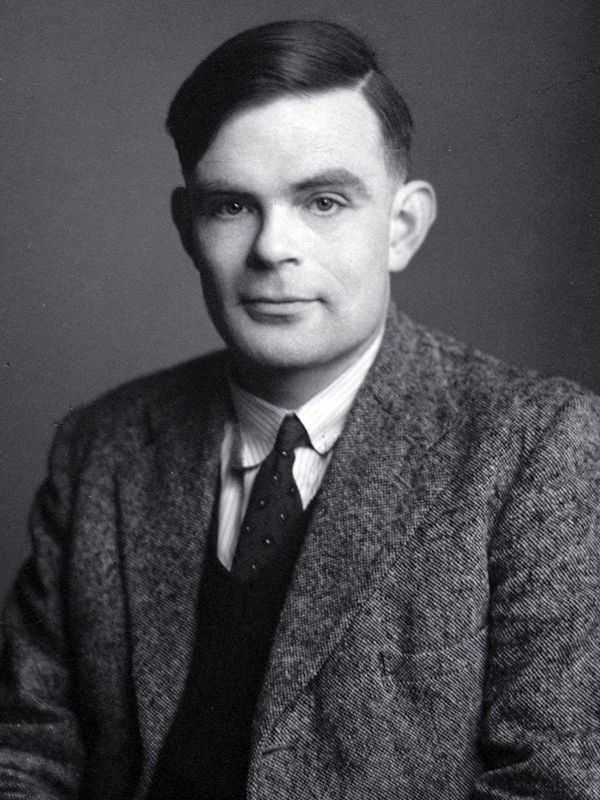
\includegraphics[width=9cm,height=9cm]{img/alan-turing.jpg}};


%Connections
\draw [connection]  (c1-east)   -- node {\midarrow} (p1-west);
\draw[->, densely dashed]
(c1-nearnortheast) -- (p1-nearnorthwest)
(c1-nearsoutheast) -- (p1-nearsouthwest)
(c1-farsoutheast)  -- (p1-farsouthwest)
(c1-farnortheast)  -- (p1-farnorthwest)
;
\draw [connection]  (p1-east)   -- node {\midarrow} (c2-west);
\draw[densely dashed]
(p1-nearnortheast) -- (c2-nearnorthwest)
(p1-nearsoutheast) -- (c2-nearsouthwest)
(p1-farsoutheast)  -- (c2-farsouthwest)
(p1-farnortheast)  -- (c2-farnorthwest)
;
\draw [connection]  (p2-east)   -- node {\midarrow} (c3-west);
\draw[densely dashed]
(p2-nearnortheast) -- (c3-nearnorthwest)
(p2-nearsoutheast) -- (c3-nearsouthwest)
(p2-farsoutheast)  -- (c3-farsouthwest)
(p2-farnortheast)  -- (c3-farnorthwest)
;

\draw [connection]  (c2-east)   -- node {\midarrow} (p2-west);
\draw[densely dashed]
(c2-nearnortheast) -- (p2-nearnorthwest)
(c2-nearsoutheast) -- (p2-nearsouthwest)
(c2-farsoutheast)  -- (p2-farsouthwest)
(c2-farnortheast)  -- (p2-farnorthwest)
;
\draw [connection]  (c3-east)   -- node {\midarrow} (up1-west);
\draw[densely dashed]
(c3-nearnortheast) -- (up1-nearnorthwest)
(c3-nearsoutheast) -- (up1-nearsouthwest)
(c3-farsoutheast)  -- (up1-farsouthwest)
(c3-farnortheast)  -- (up1-farnorthwest)
;
\draw [connection]  (c4-east)   -- node {\midarrow} (up2-west);
\draw[densely dashed]
(c4-nearnortheast) -- (up2-nearnorthwest)
(c4-nearsoutheast) -- (up2-nearsouthwest)
(c4-farsoutheast)  -- (up2-farsouthwest)
(c4-farnortheast)  -- (up2-farnorthwest)
;
\draw [connection]  (up1-east)   -- node {\midarrow} (c4-west);
\draw[densely dashed]
(up1-nearnortheast) -- (c4-nearnorthwest)
(up1-nearsoutheast) -- (c4-nearsouthwest)
(up1-farsoutheast)  -- (c4-farsouthwest)
(up1-farnortheast)  -- (c4-farnorthwest)
;
\draw [connection]  (up2-east)   -- node {\midarrow} (c5-west);
\draw[densely dashed]
(up2-nearnortheast) -- (c5-nearnorthwest)
(up2-nearsoutheast) -- (c5-nearsouthwest)
(up2-farsoutheast)  -- (c5-farsouthwest)
(up2-farnortheast)  -- (c5-farnorthwest)
;


\end{tikzpicture}
\end{document}\grid
